\documentclass[a4paper,11pt]{article}

% Kodovani (cestiny) v dokumentu: utf-8
%\usepackage[cp1250]{inputenc}	% Omezena stredoevropska kodova stranka, pouze MSW.
\usepackage[utf8]{inputenc}	% Doporucujeme pouzivat UTF-8 (unicode).

\usepackage[margin=2cm]{geometry}
\newtoks\jmenopraktika \newtoks\jmeno \newtoks\datum
\newtoks\obor \newtoks\skupina \newtoks\rocnik \newtoks\semestr
\newtoks\cisloulohy \newtoks\jmenoulohy
\newtoks\tlak \newtoks\teplota \newtoks\vlhkost

\jmenopraktika={Fyzikální praktikum 2}
\jmeno={Lukáš Lejdar}
\datum={12. listopadu 2024}
\obor={F}
\skupina={Út 16:00}

\cisloulohy={12}
\jmenoulohy={Optická spektroskopie}

\tlak={101{,}35}
\teplota={21,1}
\vlhkost={47,7}


%%%%%%%%%%% Uzitecne balicky:
\usepackage[czech]{babel}

\usepackage{graphicx}
\usepackage{amsmath}
\usepackage{xspace}
\usepackage{url}
\usepackage{indentfirst}
\usepackage{wrapfig}
\usepackage{xcolor}
\usepackage{subfig}
\usepackage{subcaption}
\usepackage{enumitem}
\usepackage{tikzsymbols}
\usepackage{newfloat}

\DeclareFloatingEnvironment[fileext=lof]{graph}
\captionsetup[graph]{labelformat=simple, labelsep=colon, name=Graf}

%%%%%% Zamezeni parchantu:
\widowpenalty 10000 \clubpenalty 10000 \displaywidowpenalty 10000
%%%%%% Parametry pro moznost vsazeni vetsiho poctu obrazku na stranku
\setcounter{topnumber}{3}	  % max. pocet floatu nahore (specifikace t)
\setcounter{bottomnumber}{3}	  % max. pocet floatu dole (specifikace b)
\setcounter{totalnumber}{6}	  % max. pocet floatu na strance celkem
\renewcommand\topfraction{0.9}	  % max podil stranky pro floaty nahore
\renewcommand\bottomfraction{0.9} % max podil stranky pro floaty dole
\renewcommand\textfraction{0.1}	  % min podil stranky, ktery musi obsahovat text
\intextsep=8mm \textfloatsep=8mm  %\intextsep pro ulozeni [h] floatu a \textfloatsep pro [b] or [t]

% Tecky za cisly sekci:
\renewcommand{\thesection}{\arabic{section}.}
\renewcommand{\thesubsection}{\thesection\arabic{subsection}.}
% Jednopismenna mezera mezi cislem a nazvem kapitoly:
\makeatletter \def\@seccntformat#1{\csname the#1\endcsname\hspace{1ex}} \makeatother
%
\newcommand{\vsn}[4]{\ensuremath{#1 =} #2(#3)\,#4}
\newcommand{\vrn}[6]{\ensuremath{#1 =} (#2 $\pm$ #3)\,#4 ($p=$ #5\,\%, $\nu=$ #6)}

\newcommand*\circled[1]{\tikz[baseline=(char.base)]{
		\node[shape=circle,draw,inner sep=1pt] (char) {#1};}}

%%%%%%%%%%%%%%%%%%%%%%%%%%%%%%%%%%%%%%%%%%%%%%%%%%%%%%%%%%%%%%%%%%%%%%%%%%%%%%%
% Zacatek dokumentu
%%%%%%%%%%%%%%%%%%%%%%%%%%%%%%%%%%%%%%%%%%%%%%%%%%%%%%%%%%%%%%%%%%%%%%%%%%%%%%%

\begin{document}

\thispagestyle{empty}

{
\begin{center}
\sf 
{\Large Ústav fyziky a technologií plazmatu Přírodovědecké fakulty Masarykovy univerzity} \\
\bigskip
{\huge \bfseries FYZIKÁLNÍ PRAKTIKUM} \\
\bigskip
{\Large \the\jmenopraktika}
\end{center}

\bigskip

\sf
\noindent
\setlength{\arrayrulewidth}{1pt}
\begin{tabular*}{\textwidth}{@{\extracolsep{\fill}} l l}
\large {\bfseries Zpracoval:}  \the\jmeno & \large  {\bfseries Naměřeno:} \the\datum\\[2mm]
\large  {\bfseries Obor:} \the\obor  \hspace{40mm}  {\bfseries Skupina:} \the\skupina %
&\large {\bfseries Testováno:}\\
\\
\hline
\end{tabular*}
}

\bigskip

{
\sf
\noindent \begin{tabular}{p{4cm} p{0.6\textwidth}}
\Large  Úloha č. {\bfseries \the\cisloulohy:} \par
\smallskip
$T=\the\teplota$~$^\circ$C \par
$p=\the\tlak$~kPa \par
$\varphi=\the\vlhkost$~\%
&\Large \bfseries \the\jmenoulohy  \\[2mm]
\end{tabular}
}

\vskip1cm

\section{Úvod}

Cílem úlohy je změřit spektrální závislost indexu lomu a tloušťku tenké vrstvy pomocí propustnosti substrátu a v druhé části potom ověřit Lambertův-Beerův zákon pro průhledné školní pravítko a zjisit absorpční koeficienty.
 
\section{Postup měření}

\subsection{Měření spektrální závislosti indexu lomu neabsorbující tlusté vrstvy z její propustnosti}

Při průchodu paprsku světla vrstvou substrátu se část světla odrazí a dojde k relativnímu snížení jeho intenzity, kterou definujeme jako propustnost

\begin{equation}
T_s = \frac{I_1}{I_0}.
\end{equation}

Pokud je substrát neabsorbující, bude tato veličina záviset pouze na indexu lomu okolí $ n_0 $ a vzorku $ n_1 $. V případě, že paprsek dopadá kolmo na substrát a vrstva je dost široká aby nedocházelo k interferenci, platí

\begin{equation}
T_s = \frac{2n_s n_0}{n_0^2 + n_s^2}
\end{equation}

V praktiku je spektrometr, který za těchto podmínek měří spektrální propustnost $ T_s(\lambda) $ libovolného vzorku odkud ze vztahu $ 2 $ dostáváme závislost $ n_s(\lambda) $ pokud $ n_0 = 1 $.

\begin{equation}
n_s = \frac{1 + \sqrt{1 - T_s^2} }{T_s}
\end{equation}

Obdržená spektrální závislost se typicky dál analyzuje různými fyzikálními modely. Jeden z nejjednodušších je Cauchyova rovnice aproximující index lomu v oblasti bez absorbce

\begin{equation}
n(\lambda) = A + \frac{B}{\lambda^2}
\end{equation}

\subsection{Určení indexu lomu a tloušťky tenké vrstvy}

V případě měření indexu lomu tenké vrstvy jde použít podobný postup, ale bude nutné navíc započítat interferenci odražených paprsků od rozhraní. Další komplikace je, že tenká vrstva musí být kvůli své křehkosti nanesena na nějaký jiný materiál a změřená propustnost bude způsobena průchodem oběma těmito vrstvami. Z Fresnelových rovnic lze odvodit, že propustnost po průchodu takovýmto vzorkem se řídí vztahem

\begin{equation}
T_{vs} = \frac{2 n_s}{ 1 + n_s^2 + \frac{n_v^2 - 1}{2}(1 - \frac{n_s}{n_v}^2) \sin^2(\beta) }
\end{equation}

\noindent
kde $ n_s $ je index lomu tlustého substrátu a $ n_v $ index lomu tenké vrstvy. Při kolmém dopadu v neabsorbující vrstvě o šířce $ d $ je fázový faktor

\begin{equation}
\beta = 2 \pi n_v \frac{d}{\lambda}
\end{equation}

Pro získání závislost $ n_v(\lambda) $ dosadím do vztahu (6) za oba indexy lomu Cauchyovu rovnici a budu fitovat její parametry a tloušťku vrstvy $ d $.

\subsection{Lambertův-Beerův zákon a absorpční koeficient}

Pokud záření prochází absorbující tlustou vrstvou, bude jeho intenzita exponenciálně klesat s uraženou vzdáleností a absorpčním koeficientem $ \alpha $

\begin{equation}
T \propto e^{-\alpha d}.
\end{equation}

Když by navíc měl materiál velmi nízkou odrazivost, bude veškerý úbytek v intenzitě způsobený absorbcí a vztah (7) se zredukuje na

\begin{equation}
T = e^{-\alpha d}.
\end{equation}

Pro ověření tohoto vztahu použiju sérii destiček, které na sebe budu postupně skládat a měřit jejich propustnost.

\newpage

\section{Výsledky měření}

\subsection{Měření indexu lomu skla BK7}

Pomocí spektrometru Specord 40 jsem změřil spektrální závislost propustnosti vzorku skla BK7 a pomocí vztahu (3) dopočítal odpovídající indexy lomu. Tuto závislost jsem proložil Cauchyovou rovnicí a získal parametry

\vspace{-5pt}

\begin{align*}
    A &= 1.5010 \pm 0.0003 \\
    B &= 0.0068 \pm 0.0001 \ \mu \text{m} ^2
\end{align*}

\vspace{-10pt}

\begin{table}[htpb]
    \begin{minipage}[b]{.5\linewidth}
        \centering
        \resizebox{\textwidth}{!}{ % GNUPLOT: LaTeX picture with Postscript
\begingroup
  \makeatletter
  \providecommand\color[2][]{%
    \GenericError{(gnuplot) \space\space\space\@spaces}{%
      Package color not loaded in conjunction with
      terminal option `colourtext'%
    }{See the gnuplot documentation for explanation.%
    }{Either use 'blacktext' in gnuplot or load the package
      color.sty in LaTeX.}%
    \renewcommand\color[2][]{}%
  }%
  \providecommand\includegraphics[2][]{%
    \GenericError{(gnuplot) \space\space\space\@spaces}{%
      Package graphicx or graphics not loaded%
    }{See the gnuplot documentation for explanation.%
    }{The gnuplot epslatex terminal needs graphicx.sty or graphics.sty.}%
    \renewcommand\includegraphics[2][]{}%
  }%
  \providecommand\rotatebox[2]{#2}%
  \@ifundefined{ifGPcolor}{%
    \newif\ifGPcolor
    \GPcolorfalse
  }{}%
  \@ifundefined{ifGPblacktext}{%
    \newif\ifGPblacktext
    \GPblacktexttrue
  }{}%
  % define a \g@addto@macro without @ in the name:
  \let\gplgaddtomacro\g@addto@macro
  % define empty templates for all commands taking text:
  \gdef\gplbacktext{}%
  \gdef\gplfronttext{}%
  \makeatother
  \ifGPblacktext
    % no textcolor at all
    \def\colorrgb#1{}%
    \def\colorgray#1{}%
  \else
    % gray or color?
    \ifGPcolor
      \def\colorrgb#1{\color[rgb]{#1}}%
      \def\colorgray#1{\color[gray]{#1}}%
      \expandafter\def\csname LTw\endcsname{\color{white}}%
      \expandafter\def\csname LTb\endcsname{\color{black}}%
      \expandafter\def\csname LTa\endcsname{\color{black}}%
      \expandafter\def\csname LT0\endcsname{\color[rgb]{1,0,0}}%
      \expandafter\def\csname LT1\endcsname{\color[rgb]{0,1,0}}%
      \expandafter\def\csname LT2\endcsname{\color[rgb]{0,0,1}}%
      \expandafter\def\csname LT3\endcsname{\color[rgb]{1,0,1}}%
      \expandafter\def\csname LT4\endcsname{\color[rgb]{0,1,1}}%
      \expandafter\def\csname LT5\endcsname{\color[rgb]{1,1,0}}%
      \expandafter\def\csname LT6\endcsname{\color[rgb]{0,0,0}}%
      \expandafter\def\csname LT7\endcsname{\color[rgb]{1,0.3,0}}%
      \expandafter\def\csname LT8\endcsname{\color[rgb]{0.5,0.5,0.5}}%
    \else
      % gray
      \def\colorrgb#1{\color{black}}%
      \def\colorgray#1{\color[gray]{#1}}%
      \expandafter\def\csname LTw\endcsname{\color{white}}%
      \expandafter\def\csname LTb\endcsname{\color{black}}%
      \expandafter\def\csname LTa\endcsname{\color{black}}%
      \expandafter\def\csname LT0\endcsname{\color{black}}%
      \expandafter\def\csname LT1\endcsname{\color{black}}%
      \expandafter\def\csname LT2\endcsname{\color{black}}%
      \expandafter\def\csname LT3\endcsname{\color{black}}%
      \expandafter\def\csname LT4\endcsname{\color{black}}%
      \expandafter\def\csname LT5\endcsname{\color{black}}%
      \expandafter\def\csname LT6\endcsname{\color{black}}%
      \expandafter\def\csname LT7\endcsname{\color{black}}%
      \expandafter\def\csname LT8\endcsname{\color{black}}%
    \fi
  \fi
    \setlength{\unitlength}{0.0500bp}%
    \ifx\gptboxheight\undefined%
      \newlength{\gptboxheight}%
      \newlength{\gptboxwidth}%
      \newsavebox{\gptboxtext}%
    \fi%
    \setlength{\fboxrule}{0.5pt}%
    \setlength{\fboxsep}{1pt}%
    \definecolor{tbcol}{rgb}{1,1,1}%
\begin{picture}(5760.00,4320.00)%
    \gplgaddtomacro\gplbacktext{%
      \csname LTb\endcsname%%
      \put(386,704){\makebox(0,0)[r]{\strut{}$89$}}%
      \put(386,1189){\makebox(0,0)[r]{\strut{}$89.5$}}%
      \put(386,1674){\makebox(0,0)[r]{\strut{}$90$}}%
      \put(386,2159){\makebox(0,0)[r]{\strut{}$90.5$}}%
      \put(386,2644){\makebox(0,0)[r]{\strut{}$91$}}%
      \put(386,3129){\makebox(0,0)[r]{\strut{}$91.5$}}%
      \put(386,3614){\makebox(0,0)[r]{\strut{}$92$}}%
      \put(386,4099){\makebox(0,0)[r]{\strut{}$92.5$}}%
      \put(881,484){\makebox(0,0){\strut{}$400$}}%
      \put(1608,484){\makebox(0,0){\strut{}$500$}}%
      \put(2334,484){\makebox(0,0){\strut{}$600$}}%
      \put(3061,484){\makebox(0,0){\strut{}$700$}}%
      \put(3787,484){\makebox(0,0){\strut{}$800$}}%
      \put(4514,484){\makebox(0,0){\strut{}$900$}}%
      \put(5240,484){\makebox(0,0){\strut{}$1000$}}%
    }%
    \gplgaddtomacro\gplfronttext{%
      \csname LTb\endcsname%%
      \put(-351,2401){\rotatebox{-270.00}{\makebox(0,0){\strut{}propustnost \%}}}%
      \put(2879,154){\makebox(0,0){\strut{}$\lambda$ (nm)}}%
    }%
    \gplbacktext
    \put(0,0){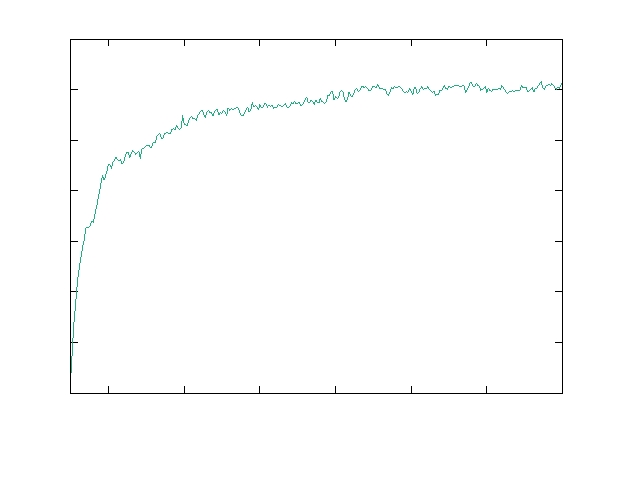
\includegraphics[width={288.00bp},height={216.00bp}]{bk7}}%
    \gplfronttext
  \end{picture}%
\endgroup
 }
    \end{minipage} 
    \hfill
    \begin{minipage}[b]{.5\linewidth}
        \centering
        \resizebox{\textwidth}{!}{ % GNUPLOT: LaTeX picture with Postscript
\begingroup
  \makeatletter
  \providecommand\color[2][]{%
    \GenericError{(gnuplot) \space\space\space\@spaces}{%
      Package color not loaded in conjunction with
      terminal option `colourtext'%
    }{See the gnuplot documentation for explanation.%
    }{Either use 'blacktext' in gnuplot or load the package
      color.sty in LaTeX.}%
    \renewcommand\color[2][]{}%
  }%
  \providecommand\includegraphics[2][]{%
    \GenericError{(gnuplot) \space\space\space\@spaces}{%
      Package graphicx or graphics not loaded%
    }{See the gnuplot documentation for explanation.%
    }{The gnuplot epslatex terminal needs graphicx.sty or graphics.sty.}%
    \renewcommand\includegraphics[2][]{}%
  }%
  \providecommand\rotatebox[2]{#2}%
  \@ifundefined{ifGPcolor}{%
    \newif\ifGPcolor
    \GPcolorfalse
  }{}%
  \@ifundefined{ifGPblacktext}{%
    \newif\ifGPblacktext
    \GPblacktexttrue
  }{}%
  % define a \g@addto@macro without @ in the name:
  \let\gplgaddtomacro\g@addto@macro
  % define empty templates for all commands taking text:
  \gdef\gplbacktext{}%
  \gdef\gplfronttext{}%
  \makeatother
  \ifGPblacktext
    % no textcolor at all
    \def\colorrgb#1{}%
    \def\colorgray#1{}%
  \else
    % gray or color?
    \ifGPcolor
      \def\colorrgb#1{\color[rgb]{#1}}%
      \def\colorgray#1{\color[gray]{#1}}%
      \expandafter\def\csname LTw\endcsname{\color{white}}%
      \expandafter\def\csname LTb\endcsname{\color{black}}%
      \expandafter\def\csname LTa\endcsname{\color{black}}%
      \expandafter\def\csname LT0\endcsname{\color[rgb]{1,0,0}}%
      \expandafter\def\csname LT1\endcsname{\color[rgb]{0,1,0}}%
      \expandafter\def\csname LT2\endcsname{\color[rgb]{0,0,1}}%
      \expandafter\def\csname LT3\endcsname{\color[rgb]{1,0,1}}%
      \expandafter\def\csname LT4\endcsname{\color[rgb]{0,1,1}}%
      \expandafter\def\csname LT5\endcsname{\color[rgb]{1,1,0}}%
      \expandafter\def\csname LT6\endcsname{\color[rgb]{0,0,0}}%
      \expandafter\def\csname LT7\endcsname{\color[rgb]{1,0.3,0}}%
      \expandafter\def\csname LT8\endcsname{\color[rgb]{0.5,0.5,0.5}}%
    \else
      % gray
      \def\colorrgb#1{\color{black}}%
      \def\colorgray#1{\color[gray]{#1}}%
      \expandafter\def\csname LTw\endcsname{\color{white}}%
      \expandafter\def\csname LTb\endcsname{\color{black}}%
      \expandafter\def\csname LTa\endcsname{\color{black}}%
      \expandafter\def\csname LT0\endcsname{\color{black}}%
      \expandafter\def\csname LT1\endcsname{\color{black}}%
      \expandafter\def\csname LT2\endcsname{\color{black}}%
      \expandafter\def\csname LT3\endcsname{\color{black}}%
      \expandafter\def\csname LT4\endcsname{\color{black}}%
      \expandafter\def\csname LT5\endcsname{\color{black}}%
      \expandafter\def\csname LT6\endcsname{\color{black}}%
      \expandafter\def\csname LT7\endcsname{\color{black}}%
      \expandafter\def\csname LT8\endcsname{\color{black}}%
    \fi
  \fi
    \setlength{\unitlength}{0.0500bp}%
    \ifx\gptboxheight\undefined%
      \newlength{\gptboxheight}%
      \newlength{\gptboxwidth}%
      \newsavebox{\gptboxtext}%
    \fi%
    \setlength{\fboxrule}{0.5pt}%
    \setlength{\fboxsep}{1pt}%
    \definecolor{tbcol}{rgb}{1,1,1}%
\begin{picture}(5760.00,4320.00)%
    \gplgaddtomacro\gplbacktext{%
      \csname LTb\endcsname%%
      \put(386,704){\makebox(0,0)[r]{\strut{}$1.5$}}%
      \put(386,1189){\makebox(0,0)[r]{\strut{}$1.52$}}%
      \put(386,1674){\makebox(0,0)[r]{\strut{}$1.54$}}%
      \put(386,2159){\makebox(0,0)[r]{\strut{}$1.56$}}%
      \put(386,2644){\makebox(0,0)[r]{\strut{}$1.58$}}%
      \put(386,3129){\makebox(0,0)[r]{\strut{}$1.6$}}%
      \put(386,3614){\makebox(0,0)[r]{\strut{}$1.62$}}%
      \put(386,4099){\makebox(0,0)[r]{\strut{}$1.64$}}%
      \put(881,484){\makebox(0,0){\strut{}$400$}}%
      \put(1608,484){\makebox(0,0){\strut{}$500$}}%
      \put(2334,484){\makebox(0,0){\strut{}$600$}}%
      \put(3061,484){\makebox(0,0){\strut{}$700$}}%
      \put(3787,484){\makebox(0,0){\strut{}$800$}}%
      \put(4514,484){\makebox(0,0){\strut{}$900$}}%
      \put(5240,484){\makebox(0,0){\strut{}$1000$}}%
    }%
    \gplgaddtomacro\gplfronttext{%
      \csname LTb\endcsname%%
      \put(4253,3926){\makebox(0,0)[r]{\strut{}fit}}%
      \csname LTb\endcsname%%
      \put(-351,2401){\rotatebox{-270.00}{\makebox(0,0){\strut{}$n_s$}}}%
      \put(2879,154){\makebox(0,0){\strut{}$\lambda$ (nm)}}%
    }%
    \gplbacktext
    \put(0,0){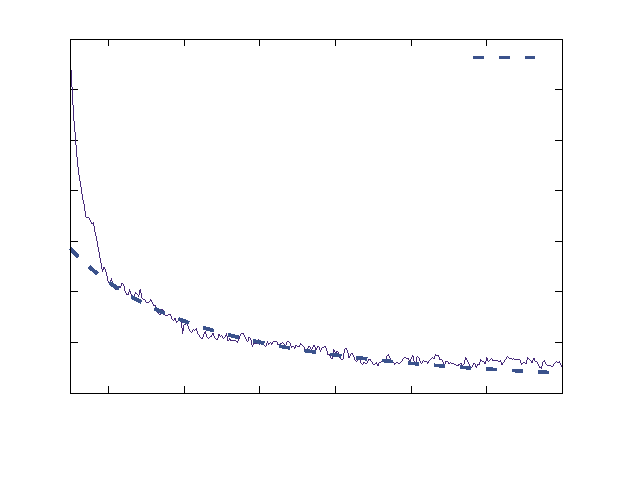
\includegraphics[width={288.00bp},height={216.00bp}]{bk7_n}}%
    \gplfronttext
  \end{picture}%
\endgroup
 }
    \end{minipage} 
    \captionsetup{type=graph}
    \caption{Závislosti propustnosti a indexu lomu destičky optického skla BK7 na vlnové délce}
\end{table}

\subsection{Měření indexu lomu tenké vrstvy a její tloušťky}

Změřil jsem spektrální propustnost vzorku skla BK7 s tenkou vrstvou z oxidu titaničitého a hodnoty fitoval vztahem (6), po dosazení Cauchyovy rovnice (4) za oba indexy lomu. Změřené hodnoty jsem vynesl do grafů 2 a níže uvedl získané parametry fitu.

\vspace{-5pt}

\begin{align*}
    A_s &= (1.50 \pm 0.01) & A_v &= (2.22 \pm 0.004) & d  &= (524.9 \pm 0.9) \ \text{nm}\\
    B_s &= (0.022 \pm 0.004)  \ \mu \text{m} ^2  & B_v &= (0.0626 \pm 0.0005) \ \mu \text{m} ^2
\end{align*}

\vspace{-10pt}

\begin{table}[htpb]
    \begin{minipage}[b]{.625\linewidth}
        \centering
        \resizebox{\textwidth}{!}{ % GNUPLOT: LaTeX picture with Postscript
\begingroup
  \makeatletter
  \providecommand\color[2][]{%
    \GenericError{(gnuplot) \space\space\space\@spaces}{%
      Package color not loaded in conjunction with
      terminal option `colourtext'%
    }{See the gnuplot documentation for explanation.%
    }{Either use 'blacktext' in gnuplot or load the package
      color.sty in LaTeX.}%
    \renewcommand\color[2][]{}%
  }%
  \providecommand\includegraphics[2][]{%
    \GenericError{(gnuplot) \space\space\space\@spaces}{%
      Package graphicx or graphics not loaded%
    }{See the gnuplot documentation for explanation.%
    }{The gnuplot epslatex terminal needs graphicx.sty or graphics.sty.}%
    \renewcommand\includegraphics[2][]{}%
  }%
  \providecommand\rotatebox[2]{#2}%
  \@ifundefined{ifGPcolor}{%
    \newif\ifGPcolor
    \GPcolortrue
  }{}%
  \@ifundefined{ifGPblacktext}{%
    \newif\ifGPblacktext
    \GPblacktextfalse
  }{}%
  % define a \g@addto@macro without @ in the name:
  \let\gplgaddtomacro\g@addto@macro
  % define empty templates for all commands taking text:
  \gdef\gplbacktext{}%
  \gdef\gplfronttext{}%
  \makeatother
  \ifGPblacktext
    % no textcolor at all
    \def\colorrgb#1{}%
    \def\colorgray#1{}%
  \else
    % gray or color?
    \ifGPcolor
      \def\colorrgb#1{\color[rgb]{#1}}%
      \def\colorgray#1{\color[gray]{#1}}%
      \expandafter\def\csname LTw\endcsname{\color{white}}%
      \expandafter\def\csname LTb\endcsname{\color{black}}%
      \expandafter\def\csname LTa\endcsname{\color{black}}%
      \expandafter\def\csname LT0\endcsname{\color[rgb]{1,0,0}}%
      \expandafter\def\csname LT1\endcsname{\color[rgb]{0,1,0}}%
      \expandafter\def\csname LT2\endcsname{\color[rgb]{0,0,1}}%
      \expandafter\def\csname LT3\endcsname{\color[rgb]{1,0,1}}%
      \expandafter\def\csname LT4\endcsname{\color[rgb]{0,1,1}}%
      \expandafter\def\csname LT5\endcsname{\color[rgb]{1,1,0}}%
      \expandafter\def\csname LT6\endcsname{\color[rgb]{0,0,0}}%
      \expandafter\def\csname LT7\endcsname{\color[rgb]{1,0.3,0}}%
      \expandafter\def\csname LT8\endcsname{\color[rgb]{0.5,0.5,0.5}}%
    \else
      % gray
      \def\colorrgb#1{\color{black}}%
      \def\colorgray#1{\color[gray]{#1}}%
      \expandafter\def\csname LTw\endcsname{\color{white}}%
      \expandafter\def\csname LTb\endcsname{\color{black}}%
      \expandafter\def\csname LTa\endcsname{\color{black}}%
      \expandafter\def\csname LT0\endcsname{\color{black}}%
      \expandafter\def\csname LT1\endcsname{\color{black}}%
      \expandafter\def\csname LT2\endcsname{\color{black}}%
      \expandafter\def\csname LT3\endcsname{\color{black}}%
      \expandafter\def\csname LT4\endcsname{\color{black}}%
      \expandafter\def\csname LT5\endcsname{\color{black}}%
      \expandafter\def\csname LT6\endcsname{\color{black}}%
      \expandafter\def\csname LT7\endcsname{\color{black}}%
      \expandafter\def\csname LT8\endcsname{\color{black}}%
    \fi
  \fi
    \setlength{\unitlength}{0.0500bp}%
    \ifx\gptboxheight\undefined%
      \newlength{\gptboxheight}%
      \newlength{\gptboxwidth}%
      \newsavebox{\gptboxtext}%
    \fi%
    \setlength{\fboxrule}{0.5pt}%
    \setlength{\fboxsep}{1pt}%
    \definecolor{tbcol}{rgb}{1,1,1}%
\begin{picture}(7200.00,4320.00)%
    \gplgaddtomacro\gplbacktext{%
      \csname LTb\endcsname%%
      \put(516,704){\makebox(0,0)[r]{\strut{}$30$}}%
      \put(516,1157){\makebox(0,0)[r]{\strut{}$40$}}%
      \put(516,1609){\makebox(0,0)[r]{\strut{}$50$}}%
      \put(516,2062){\makebox(0,0)[r]{\strut{}$60$}}%
      \put(516,2515){\makebox(0,0)[r]{\strut{}$70$}}%
      \put(516,2967){\makebox(0,0)[r]{\strut{}$80$}}%
      \put(516,3420){\makebox(0,0)[r]{\strut{}$90$}}%
      \put(516,3873){\makebox(0,0)[r]{\strut{}$100$}}%
      \put(1102,484){\makebox(0,0){\strut{}$400$}}%
      \put(2010,484){\makebox(0,0){\strut{}$500$}}%
      \put(2918,484){\makebox(0,0){\strut{}$600$}}%
      \put(3827,484){\makebox(0,0){\strut{}$700$}}%
      \put(4735,484){\makebox(0,0){\strut{}$800$}}%
      \put(5643,484){\makebox(0,0){\strut{}$900$}}%
      \put(6551,484){\makebox(0,0){\strut{}$1000$}}%
    }%
    \gplgaddtomacro\gplfronttext{%
      \csname LTb\endcsname%%
      \put(5564,3926){\makebox(0,0)[r]{\strut{}$T_{vs}(\lambda)$}}%
      \csname LTb\endcsname%%
      \put(5564,3706){\makebox(0,0)[r]{\strut{}fit}}%
      \csname LTb\endcsname%%
      \put(-89,2401){\rotatebox{-270.00}{\makebox(0,0){\strut{}propustnost \%}}}%
      \put(3599,154){\makebox(0,0){\strut{}$\lambda$ (nm)}}%
    }%
    \gplbacktext
    \put(0,0){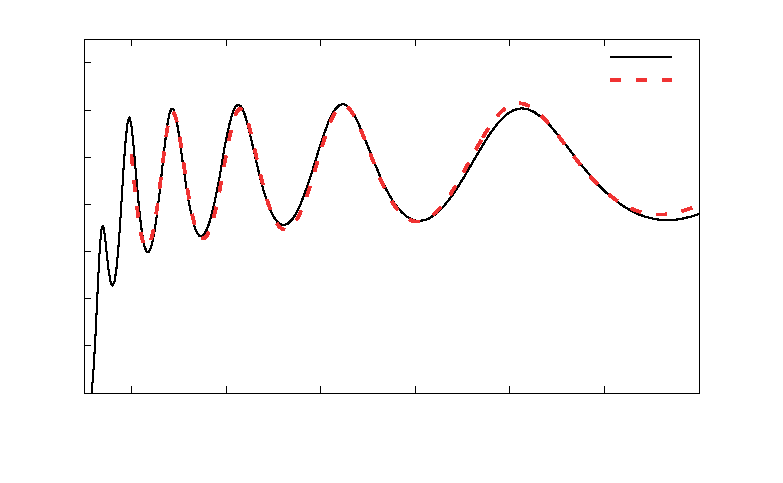
\includegraphics[width={360.00bp},height={216.00bp}]{tio2}}%
    \gplfronttext
  \end{picture}%
\endgroup
 }
    \end{minipage} 
    \hfill
    \begin{minipage}[b]{.375\linewidth}
        \centering
        \resizebox{\textwidth}{!}{ % GNUPLOT: LaTeX picture with Postscript
\begingroup
  \makeatletter
  \providecommand\color[2][]{%
    \GenericError{(gnuplot) \space\space\space\@spaces}{%
      Package color not loaded in conjunction with
      terminal option `colourtext'%
    }{See the gnuplot documentation for explanation.%
    }{Either use 'blacktext' in gnuplot or load the package
      color.sty in LaTeX.}%
    \renewcommand\color[2][]{}%
  }%
  \providecommand\includegraphics[2][]{%
    \GenericError{(gnuplot) \space\space\space\@spaces}{%
      Package graphicx or graphics not loaded%
    }{See the gnuplot documentation for explanation.%
    }{The gnuplot epslatex terminal needs graphicx.sty or graphics.sty.}%
    \renewcommand\includegraphics[2][]{}%
  }%
  \providecommand\rotatebox[2]{#2}%
  \@ifundefined{ifGPcolor}{%
    \newif\ifGPcolor
    \GPcolortrue
  }{}%
  \@ifundefined{ifGPblacktext}{%
    \newif\ifGPblacktext
    \GPblacktextfalse
  }{}%
  % define a \g@addto@macro without @ in the name:
  \let\gplgaddtomacro\g@addto@macro
  % define empty templates for all commands taking text:
  \gdef\gplbacktext{}%
  \gdef\gplfronttext{}%
  \makeatother
  \ifGPblacktext
    % no textcolor at all
    \def\colorrgb#1{}%
    \def\colorgray#1{}%
  \else
    % gray or color?
    \ifGPcolor
      \def\colorrgb#1{\color[rgb]{#1}}%
      \def\colorgray#1{\color[gray]{#1}}%
      \expandafter\def\csname LTw\endcsname{\color{white}}%
      \expandafter\def\csname LTb\endcsname{\color{black}}%
      \expandafter\def\csname LTa\endcsname{\color{black}}%
      \expandafter\def\csname LT0\endcsname{\color[rgb]{1,0,0}}%
      \expandafter\def\csname LT1\endcsname{\color[rgb]{0,1,0}}%
      \expandafter\def\csname LT2\endcsname{\color[rgb]{0,0,1}}%
      \expandafter\def\csname LT3\endcsname{\color[rgb]{1,0,1}}%
      \expandafter\def\csname LT4\endcsname{\color[rgb]{0,1,1}}%
      \expandafter\def\csname LT5\endcsname{\color[rgb]{1,1,0}}%
      \expandafter\def\csname LT6\endcsname{\color[rgb]{0,0,0}}%
      \expandafter\def\csname LT7\endcsname{\color[rgb]{1,0.3,0}}%
      \expandafter\def\csname LT8\endcsname{\color[rgb]{0.5,0.5,0.5}}%
    \else
      % gray
      \def\colorrgb#1{\color{black}}%
      \def\colorgray#1{\color[gray]{#1}}%
      \expandafter\def\csname LTw\endcsname{\color{white}}%
      \expandafter\def\csname LTb\endcsname{\color{black}}%
      \expandafter\def\csname LTa\endcsname{\color{black}}%
      \expandafter\def\csname LT0\endcsname{\color{black}}%
      \expandafter\def\csname LT1\endcsname{\color{black}}%
      \expandafter\def\csname LT2\endcsname{\color{black}}%
      \expandafter\def\csname LT3\endcsname{\color{black}}%
      \expandafter\def\csname LT4\endcsname{\color{black}}%
      \expandafter\def\csname LT5\endcsname{\color{black}}%
      \expandafter\def\csname LT6\endcsname{\color{black}}%
      \expandafter\def\csname LT7\endcsname{\color{black}}%
      \expandafter\def\csname LT8\endcsname{\color{black}}%
    \fi
  \fi
    \setlength{\unitlength}{0.0500bp}%
    \ifx\gptboxheight\undefined%
      \newlength{\gptboxheight}%
      \newlength{\gptboxwidth}%
      \newsavebox{\gptboxtext}%
    \fi%
    \setlength{\fboxrule}{0.5pt}%
    \setlength{\fboxsep}{1pt}%
    \definecolor{tbcol}{rgb}{1,1,1}%
\begin{picture}(4320.00,4320.00)%
    \gplgaddtomacro\gplbacktext{%
      \csname LTb\endcsname%%
      \put(256,704){\makebox(0,0)[r]{\strut{}$1.4$}}%
      \put(256,1189){\makebox(0,0)[r]{\strut{}$1.6$}}%
      \put(256,1674){\makebox(0,0)[r]{\strut{}$1.8$}}%
      \put(256,2159){\makebox(0,0)[r]{\strut{}$2$}}%
      \put(256,2644){\makebox(0,0)[r]{\strut{}$2.2$}}%
      \put(256,3129){\makebox(0,0)[r]{\strut{}$2.4$}}%
      \put(256,3614){\makebox(0,0)[r]{\strut{}$2.6$}}%
      \put(256,4099){\makebox(0,0)[r]{\strut{}$2.8$}}%
      \put(388,484){\makebox(0,0){\strut{}$400$}}%
      \put(978,484){\makebox(0,0){\strut{}$500$}}%
      \put(1569,484){\makebox(0,0){\strut{}$600$}}%
      \put(2159,484){\makebox(0,0){\strut{}$700$}}%
      \put(2749,484){\makebox(0,0){\strut{}$800$}}%
      \put(3340,484){\makebox(0,0){\strut{}$900$}}%
      \put(3930,484){\makebox(0,0){\strut{}$1000$}}%
    }%
    \gplgaddtomacro\gplfronttext{%
      \csname LTb\endcsname%%
      \put(2943,3926){\makebox(0,0)[r]{\strut{}fit $ n_v $}}%
      \csname LTb\endcsname%%
      \put(2943,3706){\makebox(0,0)[r]{\strut{}fit $ n_s $}}%
      \csname LTb\endcsname%%
      \put(-349,2401){\rotatebox{-270.00}{\makebox(0,0){\strut{}n}}}%
      \put(2159,154){\makebox(0,0){\strut{}$\lambda$ (nm)}}%
    }%
    \gplbacktext
    \put(0,0){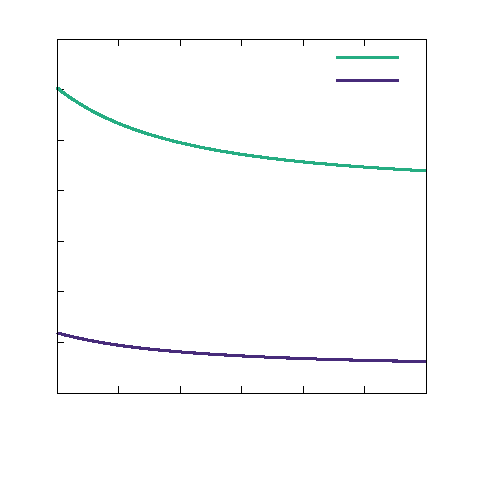
\includegraphics[width={216.00bp},height={216.00bp}]{tio2_n}}%
    \gplfronttext
  \end{picture}%
\endgroup
 }
    \end{minipage} 
    \captionsetup{type=graph}
    \caption{Závislosti propustnosti a indexu lomu vrstvy a substrátu na vlnové délce}
    \vspace{-30pt}
\end{table}

\subsection{Lambertův-Beerův zákon a absorpční koeficient}

Jako destičky jsem použil nalámané průhledné školní pravítko a postupně měřil jejich celkovou propustnost, jak byli skládané jedno na druhé. Celkem to byli čtyři měření pro čtyři různé tloušťky $ d $, které jsem pak fitoval podle vztahu (8) pro každou vlnovou délku. Naměřené hodnoty a nafitované absorpční koeficienty jsou uvedené v grafech 3 a 4.

\begin{figure}[htpb]
    \centering
    % GNUPLOT: LaTeX picture with Postscript
\begingroup
  \makeatletter
  \providecommand\color[2][]{%
    \GenericError{(gnuplot) \space\space\space\@spaces}{%
      Package color not loaded in conjunction with
      terminal option `colourtext'%
    }{See the gnuplot documentation for explanation.%
    }{Either use 'blacktext' in gnuplot or load the package
      color.sty in LaTeX.}%
    \renewcommand\color[2][]{}%
  }%
  \providecommand\includegraphics[2][]{%
    \GenericError{(gnuplot) \space\space\space\@spaces}{%
      Package graphicx or graphics not loaded%
    }{See the gnuplot documentation for explanation.%
    }{The gnuplot epslatex terminal needs graphicx.sty or graphics.sty.}%
    \renewcommand\includegraphics[2][]{}%
  }%
  \providecommand\rotatebox[2]{#2}%
  \@ifundefined{ifGPcolor}{%
    \newif\ifGPcolor
    \GPcolorfalse
  }{}%
  \@ifundefined{ifGPblacktext}{%
    \newif\ifGPblacktext
    \GPblacktexttrue
  }{}%
  % define a \g@addto@macro without @ in the name:
  \let\gplgaddtomacro\g@addto@macro
  % define empty templates for all commands taking text:
  \gdef\gplbacktext{}%
  \gdef\gplfronttext{}%
  \makeatother
  \ifGPblacktext
    % no textcolor at all
    \def\colorrgb#1{}%
    \def\colorgray#1{}%
  \else
    % gray or color?
    \ifGPcolor
      \def\colorrgb#1{\color[rgb]{#1}}%
      \def\colorgray#1{\color[gray]{#1}}%
      \expandafter\def\csname LTw\endcsname{\color{white}}%
      \expandafter\def\csname LTb\endcsname{\color{black}}%
      \expandafter\def\csname LTa\endcsname{\color{black}}%
      \expandafter\def\csname LT0\endcsname{\color[rgb]{1,0,0}}%
      \expandafter\def\csname LT1\endcsname{\color[rgb]{0,1,0}}%
      \expandafter\def\csname LT2\endcsname{\color[rgb]{0,0,1}}%
      \expandafter\def\csname LT3\endcsname{\color[rgb]{1,0,1}}%
      \expandafter\def\csname LT4\endcsname{\color[rgb]{0,1,1}}%
      \expandafter\def\csname LT5\endcsname{\color[rgb]{1,1,0}}%
      \expandafter\def\csname LT6\endcsname{\color[rgb]{0,0,0}}%
      \expandafter\def\csname LT7\endcsname{\color[rgb]{1,0.3,0}}%
      \expandafter\def\csname LT8\endcsname{\color[rgb]{0.5,0.5,0.5}}%
    \else
      % gray
      \def\colorrgb#1{\color{black}}%
      \def\colorgray#1{\color[gray]{#1}}%
      \expandafter\def\csname LTw\endcsname{\color{white}}%
      \expandafter\def\csname LTb\endcsname{\color{black}}%
      \expandafter\def\csname LTa\endcsname{\color{black}}%
      \expandafter\def\csname LT0\endcsname{\color{black}}%
      \expandafter\def\csname LT1\endcsname{\color{black}}%
      \expandafter\def\csname LT2\endcsname{\color{black}}%
      \expandafter\def\csname LT3\endcsname{\color{black}}%
      \expandafter\def\csname LT4\endcsname{\color{black}}%
      \expandafter\def\csname LT5\endcsname{\color{black}}%
      \expandafter\def\csname LT6\endcsname{\color{black}}%
      \expandafter\def\csname LT7\endcsname{\color{black}}%
      \expandafter\def\csname LT8\endcsname{\color{black}}%
    \fi
  \fi
    \setlength{\unitlength}{0.0500bp}%
    \ifx\gptboxheight\undefined%
      \newlength{\gptboxheight}%
      \newlength{\gptboxwidth}%
      \newsavebox{\gptboxtext}%
    \fi%
    \setlength{\fboxrule}{0.5pt}%
    \setlength{\fboxsep}{1pt}%
    \definecolor{tbcol}{rgb}{1,1,1}%
\begin{picture}(8640.00,3888.00)%
    \gplgaddtomacro\gplbacktext{%
      \csname LTb\endcsname%%
      \put(682,116){\makebox(0,0)[r]{\strut{}$0$}}%
      \put(682,534){\makebox(0,0)[r]{\strut{}$10$}}%
      \put(682,952){\makebox(0,0)[r]{\strut{}$20$}}%
      \put(682,1369){\makebox(0,0)[r]{\strut{}$30$}}%
      \put(682,1787){\makebox(0,0)[r]{\strut{}$40$}}%
      \put(682,2205){\makebox(0,0)[r]{\strut{}$50$}}%
      \put(682,2623){\makebox(0,0)[r]{\strut{}$60$}}%
      \put(682,3040){\makebox(0,0)[r]{\strut{}$70$}}%
      \put(682,3458){\makebox(0,0)[r]{\strut{}$80$}}%
      \put(814,-104){\makebox(0,0){\strut{}$300$}}%
      \put(1805,-104){\makebox(0,0){\strut{}$400$}}%
      \put(2795,-104){\makebox(0,0){\strut{}$500$}}%
      \put(3786,-104){\makebox(0,0){\strut{}$600$}}%
      \put(4776,-104){\makebox(0,0){\strut{}$700$}}%
      \put(5767,-104){\makebox(0,0){\strut{}$800$}}%
      \put(6757,-104){\makebox(0,0){\strut{}$900$}}%
      \put(7748,-104){\makebox(0,0){\strut{}$1000$}}%
    }%
    \gplgaddtomacro\gplfronttext{%
      \csname LTb\endcsname%%
      \put(1801,3494){\makebox(0,0)[l]{\strut{}$d = 3.55$ mm}}%
      \csname LTb\endcsname%%
      \put(1801,3274){\makebox(0,0)[l]{\strut{}$d = 7.05$ mm}}%
      \csname LTb\endcsname%%
      \put(1801,3054){\makebox(0,0)[l]{\strut{}$d = 10.55$ mm}}%
      \csname LTb\endcsname%%
      \put(1801,2834){\makebox(0,0)[l]{\strut{}$d = 14.15$ mm}}%
      \csname LTb\endcsname%%
      \put(209,1891){\rotatebox{-270.00}{\makebox(0,0){\strut{}propustnost \%}}}%
      \put(4528,-434){\makebox(0,0){\strut{}$\lambda$ (nm)}}%
    }%
    \gplbacktext
    \put(0,0){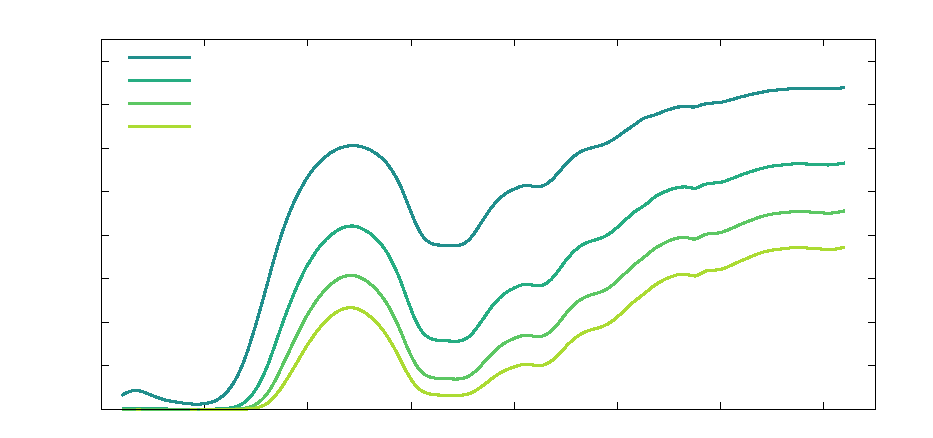
\includegraphics[width={432.00bp},height={194.40bp}]{pravitka}}%
    \gplfronttext
  \end{picture}%
\endgroup

    \captionsetup{type=graph}
    \caption{Závislost propustnosti destiček pravítka na vlnové délce pro různé výšky celkového navršení}
\end{figure}

\begin{figure}[htpb]
    \centering
    % GNUPLOT: LaTeX picture with Postscript
\begingroup
  \makeatletter
  \providecommand\color[2][]{%
    \GenericError{(gnuplot) \space\space\space\@spaces}{%
      Package color not loaded in conjunction with
      terminal option `colourtext'%
    }{See the gnuplot documentation for explanation.%
    }{Either use 'blacktext' in gnuplot or load the package
      color.sty in LaTeX.}%
    \renewcommand\color[2][]{}%
  }%
  \providecommand\includegraphics[2][]{%
    \GenericError{(gnuplot) \space\space\space\@spaces}{%
      Package graphicx or graphics not loaded%
    }{See the gnuplot documentation for explanation.%
    }{The gnuplot epslatex terminal needs graphicx.sty or graphics.sty.}%
    \renewcommand\includegraphics[2][]{}%
  }%
  \providecommand\rotatebox[2]{#2}%
  \@ifundefined{ifGPcolor}{%
    \newif\ifGPcolor
    \GPcolorfalse
  }{}%
  \@ifundefined{ifGPblacktext}{%
    \newif\ifGPblacktext
    \GPblacktexttrue
  }{}%
  % define a \g@addto@macro without @ in the name:
  \let\gplgaddtomacro\g@addto@macro
  % define empty templates for all commands taking text:
  \gdef\gplbacktext{}%
  \gdef\gplfronttext{}%
  \makeatother
  \ifGPblacktext
    % no textcolor at all
    \def\colorrgb#1{}%
    \def\colorgray#1{}%
  \else
    % gray or color?
    \ifGPcolor
      \def\colorrgb#1{\color[rgb]{#1}}%
      \def\colorgray#1{\color[gray]{#1}}%
      \expandafter\def\csname LTw\endcsname{\color{white}}%
      \expandafter\def\csname LTb\endcsname{\color{black}}%
      \expandafter\def\csname LTa\endcsname{\color{black}}%
      \expandafter\def\csname LT0\endcsname{\color[rgb]{1,0,0}}%
      \expandafter\def\csname LT1\endcsname{\color[rgb]{0,1,0}}%
      \expandafter\def\csname LT2\endcsname{\color[rgb]{0,0,1}}%
      \expandafter\def\csname LT3\endcsname{\color[rgb]{1,0,1}}%
      \expandafter\def\csname LT4\endcsname{\color[rgb]{0,1,1}}%
      \expandafter\def\csname LT5\endcsname{\color[rgb]{1,1,0}}%
      \expandafter\def\csname LT6\endcsname{\color[rgb]{0,0,0}}%
      \expandafter\def\csname LT7\endcsname{\color[rgb]{1,0.3,0}}%
      \expandafter\def\csname LT8\endcsname{\color[rgb]{0.5,0.5,0.5}}%
    \else
      % gray
      \def\colorrgb#1{\color{black}}%
      \def\colorgray#1{\color[gray]{#1}}%
      \expandafter\def\csname LTw\endcsname{\color{white}}%
      \expandafter\def\csname LTb\endcsname{\color{black}}%
      \expandafter\def\csname LTa\endcsname{\color{black}}%
      \expandafter\def\csname LT0\endcsname{\color{black}}%
      \expandafter\def\csname LT1\endcsname{\color{black}}%
      \expandafter\def\csname LT2\endcsname{\color{black}}%
      \expandafter\def\csname LT3\endcsname{\color{black}}%
      \expandafter\def\csname LT4\endcsname{\color{black}}%
      \expandafter\def\csname LT5\endcsname{\color{black}}%
      \expandafter\def\csname LT6\endcsname{\color{black}}%
      \expandafter\def\csname LT7\endcsname{\color{black}}%
      \expandafter\def\csname LT8\endcsname{\color{black}}%
    \fi
  \fi
    \setlength{\unitlength}{0.0500bp}%
    \ifx\gptboxheight\undefined%
      \newlength{\gptboxheight}%
      \newlength{\gptboxwidth}%
      \newsavebox{\gptboxtext}%
    \fi%
    \setlength{\fboxrule}{0.5pt}%
    \setlength{\fboxsep}{1pt}%
    \definecolor{tbcol}{rgb}{1,1,1}%
\begin{picture}(8640.00,3888.00)%
    \gplgaddtomacro\gplbacktext{%
      \csname LTb\endcsname%%
      \put(814,116){\makebox(0,0)[r]{\strut{}$0$}}%
      \put(814,623){\makebox(0,0)[r]{\strut{}$0.2$}}%
      \put(814,1131){\makebox(0,0)[r]{\strut{}$0.4$}}%
      \put(814,1638){\makebox(0,0)[r]{\strut{}$0.6$}}%
      \put(814,2145){\makebox(0,0)[r]{\strut{}$0.8$}}%
      \put(814,2652){\makebox(0,0)[r]{\strut{}$1$}}%
      \put(814,3160){\makebox(0,0)[r]{\strut{}$1.2$}}%
      \put(814,3667){\makebox(0,0)[r]{\strut{}$1.4$}}%
      \put(946,-104){\makebox(0,0){\strut{}$300$}}%
      \put(1919,-104){\makebox(0,0){\strut{}$400$}}%
      \put(2892,-104){\makebox(0,0){\strut{}$500$}}%
      \put(3865,-104){\makebox(0,0){\strut{}$600$}}%
      \put(4838,-104){\makebox(0,0){\strut{}$700$}}%
      \put(5811,-104){\makebox(0,0){\strut{}$800$}}%
      \put(6784,-104){\makebox(0,0){\strut{}$900$}}%
      \put(7757,-104){\makebox(0,0){\strut{}$1000$}}%
    }%
    \gplgaddtomacro\gplfronttext{%
      \csname LTb\endcsname%%
      \put(7583,3494){\makebox(0,0)[l]{\strut{}fit}}%
      \csname LTb\endcsname%%
      \put(7583,3274){\makebox(0,0)[l]{\strut{}3$ \sigma $}}%
      \csname LTb\endcsname%%
      \put(209,1891){\rotatebox{-270.00}{\makebox(0,0){\strut{}propustnost \%}}}%
      \put(4594,-434){\makebox(0,0){\strut{}$\lambda$ (nm)}}%
    }%
    \gplbacktext
    \put(0,0){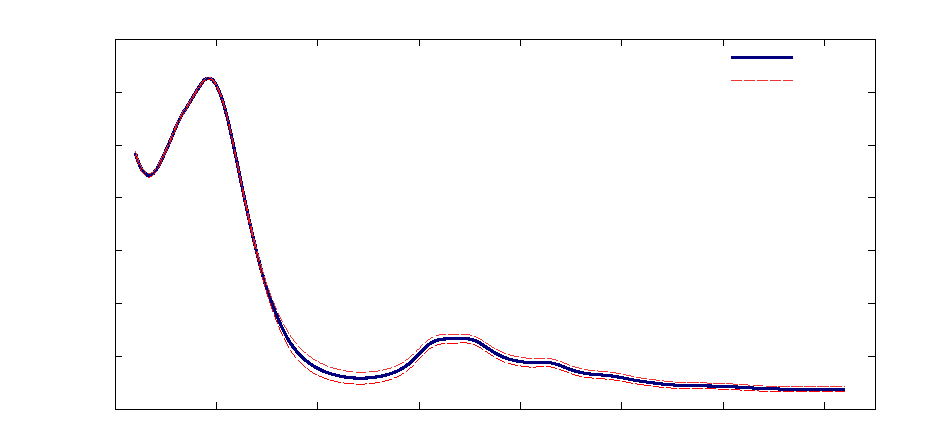
\includegraphics[width={432.00bp},height={194.40bp}]{pravitka_alphas}}%
    \gplfronttext
  \end{picture}%
\endgroup

    \captionsetup{type=graph}
    \caption{Fit koeficientů absorpce pro každou vlnovou délku}
\end{figure}

\newpage

\section{Závěr}

Z měření propustnosti skla BK7 jsem spočítal spektrální závislost indexu lomu a určil odpovídající koeficienty Cauchyovy rovnice, $ A_s = 1.5010 \pm 0.0003 $ a $ B &= 0.0068 \pm 0.0001 \ \mu \text{m} ^2 $. Tabulkové hodnoty udávají $ A_s = 1.5046 $ a $ B &= 0.00430 \ \mu \text{m} ^2 $.

Druhým vzorkem byla tenká vrstva oxidu titaničitého na substrátu skla BK7, pro kterou jsem opět změřil propustnost a tentokrát nafitoval tloušťku tenké vrstvy $ d  &= (524.9 \pm 0.9) \ \text{nm} $ a Cauchyovy koeficienty pro TiO2, $A_v &= (2.22 \pm 0.004)$ a $B_v &= (0.0626 \pm 0.0005) \ \mu \text{m} ^2$. Hodnoty vypadají správně, ale skutečné výsledky se mi nepodařilo nikde najít.

V druhé části jsem měřil propustnost vzorku s nízkou odrazivostí v závislosti na jeho tloušťce. Výsledná závislost opravdu, odpovídá Lambert-Beerovu zákonu, že intenzita prošlého světla bude klesat exponenciálně. Nafitované absorpční koeficienty v grafu 4 se totiž těší relativně nízké nejistotě.


\end{document}
